%\RequirePackage{atbegshi}
\documentclass{beamer}

\usepackage{hyperref}
\usetheme{default}
\usepackage{amssymb}
%\usepackage[cmex10]{amsmath}
\usepackage{stmaryrd}
\usepackage[english]{babel}
\usepackage{tikz,pgf,pgfplots}
\pgfplotsset{compat=newest}
\usepgflibrary{shapes,patterns}
\usepgfplotslibrary{fillbetween}
\usepgfplotslibrary{polar}
\usetikzlibrary{%
  arrows,%
  mindmap,%mindmap
  calendar,%calendar
  decorations,%decorations
  snakes,%snakes
  shapes.misc,% wg. rounded rectangle
  shapes.arrows,%
	shapes.callouts, %
  shapes,%
  chains,%
  matrix,%
  positioning,% wg. " of "
  scopes,%
  decorations.pathmorphing,% /pgf/decoration/random steps | erste Graphik
	decorations.text, %
  shadows,%
  backgrounds,%
  fit,%
  petri%
}

% Radius of regular polygons
\newdimen\R
\R=0.8cm

\definecolor{tutorial}{RGB}{50,93,61}
\definecolor{forest}{RGB}{34,139,34}
\definecolor{tamu}{RGB}{80,0,0}


\title{Estimating the Number of Active Devices \\ Within a Fixed area \\Using Wi-Fi Monitoring}
\author{Hai Li \textcolor{gray}}
\institute{Electrical and Computer Engineering \\ Texas A\&M University}
\date{ October 18, 2016}

\setbeamertemplate{footline}[page number]
\setbeamertemplate{navigation symbols}{}
%\textcolor{black}{\insertframenumber / \inserttotalframenumber}}

\newlength\tikzheight
\newlength\tikzwidth

\begin{document}

\begin{frame}
  \titlepage
\end{frame}

\begin{frame}
\frametitle{Outline}


\begin{columns}
\column{.5\textwidth}
\begin{block}{Experiential Learning}
\begin{enumerate}
\item Problem Description
\item Estimation Scheme
\item Simulation and Result
\item Experimental Implementation
\item Conclusion
\end{enumerate}
\end{block}
\end{columns}
\end{frame}

\begin{frame}
\frametitle{Notional Diagram of Inference Task}
\framesubtitle{\textcolor{gray}{\scriptsize Prof.~Gregory Huff}}
\begin{columns}
\column{.55\textwidth}
  \begin{center}
  \scalebox{0.8}{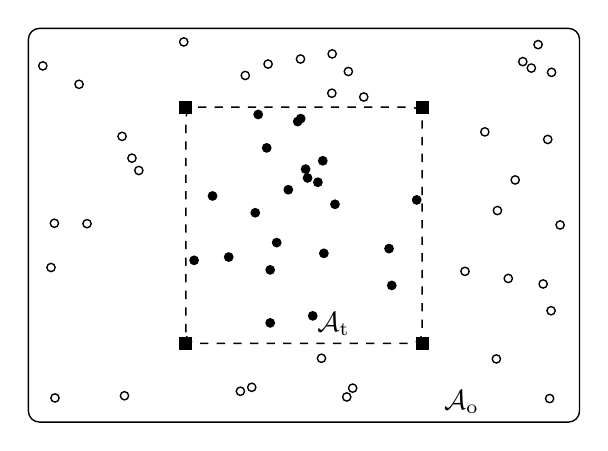
\begin{tikzpicture}
[draw=black, line width=0.5pt, inner sep=0pt,
sensor/.style={regular polygon, regular polygon sides=4, draw=black, fill=black, minimum size=6pt},
antenna/.style={ellipse, draw=none, fill=lightgray!50, minimum height=25pt, minimum width=35pt},
agent/.style={circle, draw=black, fill=black, minimum size=3pt},
outside/.style={circle, draw=black, minimum size=3pt}]

\draw[rounded corners] (0.5,0) rectangle (7.5,5);
\draw[rounded corners, dashed] (2.5,1) rectangle (5.5,4);

\node[sensor] (A1) at (2.5,1) {};
\node[sensor] (A2) at (5.5,1) {};
\node[sensor] (A3) at (5.5,4) {};
\node[sensor] (A4) at (2.5,4) {};

\node at (4.375,1.25) {$\mathcal{A}_{\mathrm{t}}$};
\node at (6,0.25) {$\mathcal{A}_{\mathrm{o}}$};


%\node[outside] at ( 2.1689410647 , 1.13775402812 ) {};
%\node[outside] at ( 2.20864248209 , 1.53164040373 ) {};
%\node[outside] at ( 2.21849793351 , 1.17616786499 ) {};
%\node[outside] at ( 2.22713611905 , 4.2883388606 ) {};
%\node[outside] at ( 2.33285623177 , 1.1314522837 ) {};
%\node[outside] at ( 2.34267400359 , 3.652875108 ) {};
\node[outside] at ( 2.47345299569 , 4.82783008639 ) {};
%\node[outside] at ( 2.51135159638 , 0.553624422059 ) {};
%\node[outside] at ( 2.52272453366 , 0.435755542295 ) {};
%\node[outside] at ( 2.89428515774 , 4.18216209512 ) {};
%\node[outside] at ( 2.49752853982 , 4.03759592194 ) {};
%\node[outside] at ( 2.51023990635 , 4.20218045094 ) {};
\node[agent] at ( 2.60516018122 , 2.05414997932 ) {};
%\node[agent] at ( 2.70214622891 , 3.55330240561 ) {};
%\node[outside] at ( 2.73317107458 , 0.543101220381 ) {};
%\node[agent] at ( 2.84935121658 , 1.15467928253 ) {};
\node[agent] at ( 2.83890584713 , 2.87152377485 ) {};
%\node[outside] at ( 2.96528485354 , 4.3464965053 ) {};
\node[outside] at ( 3.33708841304 , 0.44137061247 ) {};
\node[outside] at ( 3.19255851127 , 0.391147573008 ) {};
\node[agent] at ( 3.57135966442 , 1.25957249239 ) {};
\node[agent] at ( 3.57108996599 , 1.93263688797 ) {};
\node[agent] at ( 3.04428244813 , 2.09557253043 ) {};
\node[agent] at ( 3.65349360073 , 2.27916582855 ) {};
\node[agent] at ( 3.38165845495 , 2.65804427865 ) {};
\node[agent] at ( 3.801171656 , 2.95053880944 ) {};
\node[agent] at ( 3.52683781827 , 3.48204858325 ) {};
%\node[agent] at ( 3.11191070242 , 3.66641157636 ) {};
\node[agent] at ( 3.92046074421 , 3.81638294342 ) {};
\node[agent] at ( 3.95870651333 , 3.85414469965 ) {};
\node[agent] at ( 3.41861784707 , 3.90605027886 ) {};
\node[outside] at ( 3.25492339938 , 4.40184766792 ) {};
\node[outside] at ( 3.54457445854 , 4.54639692743 ) {};
\node[outside] at ( 3.95627386672 , 4.61065410754 ) {};
\node[outside] at ( 4.54334151472 , 0.318871863425 ) {};
\node[outside] at ( 4.61866285411 , 0.43085208228 ) {};
\node[outside] at ( 4.22256379727 , 0.810026849865 ) {};
\node[agent] at ( 4.11156281034 , 1.34890775483 ) {};
\node[agent] at ( 5.11503522961 , 1.73533325687 ) {};
\node[agent] at ( 4.25271922861 , 2.14289026089 ) {};
\node[agent] at ( 5.08072826862 , 2.20293685787 ) {};
\node[agent] at ( 4.39386727986 , 2.76582994285 ) {};
\node[agent] at ( 5.43175102407 , 2.82102596373 ) {};
\node[agent] at ( 4.17689929022 , 3.04555848331 ) {};
\node[agent] at ( 4.04574591112 , 3.10006143605 ) {};
\node[agent] at ( 4.02083927143 , 3.21271817124 ) {};
\node[agent] at ( 4.23913674945 , 3.31813256911 ) {};
%\node[agent] at ( 5.18350480449 , 3.91027292346 ) {};
\node[outside] at ( 4.7592722738 , 4.12835849149 ) {};
\node[outside] at ( 4.35389401606 , 4.17629790833 ) {};
%\node[outside] at ( 4.92106435495 , 4.30569934976 ) {};
\node[outside] at ( 4.56377465969 , 4.45205458561 ) {};
%\node[outside] at ( 5.39171408677 , 4.50063106357 ) {};
%\node[outside] at ( 5.38722123552 , 4.57106173982 ) {};
\node[outside] at ( 4.35846169798 , 4.67575131502 ) {};
%\node[outside] at ( 5.68900697359 , 4.61956803348 ) {};
%\node[outside] at ( 5.8012759141 , 0.786575025938 ) {};
\node[outside] at ( 0.683581674451 , 4.52341247559 ) {};
\node[outside] at ( 0.83059079898 , 2.52472319096 ) {};
\node[outside] at ( 0.787683048486 , 1.96310009868 ) {};
\node[outside] at ( 0.837916045306 , 0.306404502107 ) {};
%\node[outside] at ( 1.92026717467 , 3.93015374681 ) {};
%\node[outside] at ( 1.95515716802 , 4.18411686654 ) {};
\node[outside] at ( 1.81528797602 , 3.35173736185 ) {};
\node[outside] at ( 1.69019678097 , 3.6284536787 ) {};
\node[outside] at ( 1.14389478457 , 4.28971774147 ) {};
\node[outside] at ( 1.90302570449 , 3.19494880098 ) {};
\node[outside] at ( 1.2453267792 , 2.51959732965 ) {};
\node[outside] at ( 1.72075588007 , 0.334427306331 ) {};
\node[outside] at ( 6.68284689101 , 3.07494901779 ) {};
%\node[outside] at ( 6.31670524144 , 1.04082313737 ) {};
\node[outside] at ( 6.88778245976 , 4.49548052642 ) {};
%\node[outside] at ( 6.1509547887 , 1.46915491498 ) {};
\node[outside] at ( 6.04508822092 , 1.91410445168 ) {};
\node[outside] at ( 6.4571595723 , 2.68645486371 ) {};
\node[outside] at ( 6.44353320611 , 0.802163089791 ) {};
\node[outside] at ( 6.29718673575 , 3.68544388153 ) {};
\node[outside] at ( 6.97338238493 , 4.79375673213 ) {};
\node[outside] at ( 6.59506753066 , 1.82391001218 ) {};
\node[outside] at ( 6.77952439855 , 4.57765995441 ) {};
\node[outside] at ( 7.03774161105 , 1.75405750998 ) {};
\node[outside] at ( 7.1447155042 , 4.44145190374 ) {};
\node[outside] at ( 7.09582695689 , 3.58914971225 ) {};
\node[outside] at ( 7.11986402123 , 0.298547467349 ) {};
\node[outside] at ( 7.25334242268 , 2.50289493253 ) {};
\node[outside] at ( 7.13825615028 , 1.41391989682 ) {};
\end{tikzpicture}
}
  \end{center}
\column{.43\textwidth}
\begin{enumerate}
\item Monitoring devices
\item Directional antennas
\item Agents inside zone of interest
\item Agents outside area
\end{enumerate}
\end{columns}
\vfill
\begin{itemize}
  \item Periphery of target area delineated by dashed line
  \item \textbf{Estimate occupancy} inside target area
\end{itemize}
\end{frame}

\begin{frame}
\frametitle{Acquisition with Atypical Antennas}
\framesubtitle{\textcolor{gray}{\scriptsize Prof.~Gregory Huff}}
\begin{block}{\textcolor{magenta}{\textbf{Research Questions}}}
\begin{itemize}
  \item What are good designs for occupancy estimation?
  \item How should one design antennas for inference tasks?
\end{itemize}
\end{block}
\begin{center}
  \input{Figures/SignalSampling}
\end{center}
\end{frame}

\begin{frame}
\frametitle{Antenna Gain as Function of Azimuth Angle}
\framesubtitle{\textcolor{gray}{\scriptsize Hong Pan, Prof.~Gregory Huff}}
\begin{columns}
\column{.60\textwidth}
  \begin{center}
  \scalebox{0.70}{\input{Figures/SignalStrength}}
  \end{center}
\column{.38\textwidth}
\begin{block}{Experimental Setting}
  \begin{itemize}
  \item Typical devices
  \item 3 $\times$ same model
  \item $\mathrm{E}_{\theta}$-polarization\\
    $\theta = 90^{\circ}$\\
    $0^{\circ} < \phi < 360^{\circ}$
  \item Measurements obtained in TAMU anechoic chamber
  \end{itemize}
\end{block}
\end{columns}
\vfill
\begin{block}{Guideline}
  \begin{itemize}
  \item  Antenna pattern, along with device orientation, can be integrated in inference algorithm for enhanced performance.
  \end{itemize}
\end{block}
\vfill
\textcolor{gray}{\tiny ECEN~638, ECEN~626}
\end{frame}

\begin{frame}
\frametitle{Wireless Channel Characterization}
\begin{block}{Mathematical Model}
  \begin{itemize}
  \item Variations in received signal strength are governed by several factors including \textbf{mean path loss} and shadow fading
    \begin{equation*}
    P_{ij} \mathrm{[dB]}
    = A + B \log_{10} (d_{ij}) + L_{ij} + G_i(\phi_{ij})
    \end{equation*}
  \item $A$ and $B$ are mean decay parameters
  \item $d_{ij}$ represents Euclidean distance between device and monitor
  \item $L_{ij}$ denotes shadow fading
  \item $G_i (\cdot)$ is antenna gain of sensing unit
  \item Shadow fading components are independent log-normal random variables
  \end{itemize}
\end{block}
\vfill
\textcolor{gray}{\tiny ECEN~601, ECEN~683}
\end{frame}

\begin{frame}
\frametitle{Channel Characterization -- Parameter Estimation}
\framesubtitle{\textcolor{gray}{\scriptsize Daniel Tunon, Prof.~Gregory Huff}}
  \begin{center}
  \setlength\tikzheight{0.5\textwidth}
  \setlength\tikzwidth{0.8\textwidth}
  \input{Figures/LeastSquares}
  \end{center}
\end{frame}

\begin{frame}
\frametitle{Channel Parameters -- Estimation Algorithms}
\begin{itemize}
    \item Least-squares estimation infer $A$ and $B$
      \begin{align*}
      (A, B) &= \operatorname*{arg\;min}_{a,b}
      \left\| \vphantom{ \begin{bmatrix} p_1 \\ \vdots \\
      p_n \end{bmatrix}} \right.
      \underbrace{\begin{bmatrix} p_1 \\ \vdots \\
      p_n \end{bmatrix}}_{\mathbf{p}}
      - \underbrace{\begin{bmatrix} 1 & \log_{10} (d_1) \\
      \vdots & \vdots \\ 1 & \log_{10} (d_n) \end{bmatrix}}_{M}
      \begin{bmatrix} a \\ b \end{bmatrix}
      \left. \vphantom{ \begin{bmatrix} p_1 \\ \vdots \\
      p_n \end{bmatrix}} \right\|^2 \\
      &= (M^{\mathrm{H}} M)^{-1} M^{\mathrm{H}} \mathbf{p}
      \end{align*}
    \item Variance of $L$ obtained by normalizing residual error
      \begin{equation*}
      \sigma_{\mathrm{s}}^2
      = \frac{1}{(n-1)} \mathbf{p}^{\mathrm{H}}
      \left( I - M(M^{\mathrm{H}} M)^{-1} M^{\mathrm{H}} \right) \mathbf{p}
      \end{equation*}
    \item Variance of $G$ is obtained in similar fashion
\end{itemize}
\vfill
\textcolor{gray}{\tiny ECEN~601, ECEN~646, ECEN~662, STAT~611}
\end{frame}

\input{ecen2015statistics}
\input{ecen2015parallel}
\input{ecen2015iterativealgo}

\begin{frame}
\frametitle{Acquisition with Atypical Antennas (again)}
\begin{block}{\textcolor{magenta}{\textbf{Research Questions}}}
\begin{itemize}
  \item \textcolor{gray}{What are good designs for occupancy estimation?}
  \item How should one design antennas for inference tasks?
\end{itemize}
\end{block}
\begin{center}
  \input{Figures/SignalSampling}
\end{center}
\end{frame}

\begin{frame}
\frametitle{Antenna Gain as Function of Azimuth Angle}
\framesubtitle{\textcolor{gray}{\scriptsize Pranay Eedara, Hai Li, Anudeep Tungala, Nagaraj Janakiraman}}
\begin{columns}
\column{.6\textwidth}
  \begin{center}
  \scalebox{0.70}{\input{Figures/SignalStrength2}}
  \end{center}
\column{.38\textwidth}
\begin{block}{Antenna Model}
  \begin{itemize}
  \item Direction (boresight)
  \item 3~dB beamwidth
  \item $\mathrm{E}_{\theta}$-polarization\\
    $\theta = 90^{\circ}$\\
    $0^{\circ} < \phi < 360^{\circ}$
  \item Asymmetrical radiation pattern
  \end{itemize}
\end{block}
\end{columns}
\vfill
\begin{block}{Established 3GPP Antenna Model}
  \begin{itemize}
  \item Antenna radiation pattern is characterized by pointing direction of maximum gain and beamwidth
  \end{itemize}
\end{block}
\end{frame}

\begin{frame}
\frametitle{Simulation Results: Isotropic versus Directional}
\framesubtitle{\textcolor{gray}{\scriptsize Pranay Eedara, Hai Li, Anudeep Tungala, Nagaraj Janakiraman}}
\begin{columns}
\column{.6\textwidth}
  \begin{center}
  \scalebox{0.65}{\input{Figures/bmse16}}
  \end{center}
\column{.38\textwidth}
  \begin{itemize}
  \item ML estimation
  \item \textbf{Intensity} $\lambda = 16$
  \item 101 values of $\alpha$
  \item 10,000 trials per point
  \item Numerical integration based on $100 \times 100$ grid
  \end{itemize}
\end{columns}
\vfill
\begin{block}{Research Outcome}
  \begin{itemize}
  \item Directional antennas outperform isotropic system
  \item RF design considerations are significantly different for inference when compared to wireless communication
  \end{itemize}
\end{block}
\end{frame}

\begin{frame}
\frametitle{Simulation Results: Isotropic versus Directional}
\framesubtitle{\textcolor{gray}{\scriptsize Pranay Eedara, Hai Li, Anudeep Tungala, Nagaraj Janakiraman}}
\begin{columns}
\column{.6\textwidth}
  \begin{center}
  \scalebox{0.65}{\input{Figures/bmse64}}
  \end{center}
\column{.38\textwidth}
  \begin{itemize}
  \item ML estimation
  \item \textbf{Intensity} $\lambda = 64$
  \item 101 values of $\alpha$
  \item 10,000 trials per point
  \item Numerical integration based on $100 \times 100$ grid
  \end{itemize}
\end{columns}
\vfill
\begin{block}{Research Outcome}
  \begin{itemize}
  \item Directional antennas outperform isotropic system
  \item RF design considerations are significantly different for inference when compared to wireless communication
  \end{itemize}
\end{block}
\end{frame}

\begin{frame}
\frametitle{Architecture of Physical Experiment}
\framesubtitle{\textcolor{gray}{\scriptsize Pranay Eedara, Hai Li, Anudeep Tungala, Nagaraj Janakiraman}}
\begin{center}
  \includegraphics[width=0.35\textwidth]{Figures/nuc.jpg}
\end{center}
\begin{itemize}
\item Experimental setup consists of three components
  \begin{itemize}
  \item Alpha network card AWUS036NHA
  \item Local processing units: Intel Next Unit of Computing
  \item Cloud server
  \end{itemize}
\item NIC operates in monitor mode to capture WiFi packets
\item Local processing units parses information: MAC addresses, RSSI values, time stamps
\item Central server aggregates data from monitoring devices
\item RSSI values are employed as basis for inference
 \end{itemize}
\end{frame}

\begin{frame}
\frametitle{Architecture of Physical Experiment}
\framesubtitle{\textcolor{gray}{\scriptsize Pranay Eedara, Hai Li, Anudeep Tungala, Nagaraj Janakiraman}}
\begin{center}
  \includegraphics[width=0.6\textwidth]{Figures/qrcode.png}
\end{center}
\begin{center}
    \url{https://plot.ly/~epranaykumar/29.embed}
\end{center}
\end{frame}

\input{ecen2015graph}

\begin{frame}
\frametitle{Acquisition with Reconfigurable Antennas}
\begin{block}{\textcolor{magenta}{\textbf{Research Opportunity}}}
\begin{itemize}
  \item Distinct antenna configurations create additional samples
  \item Reconfigurable system is statistically superior
  \item Design of reconfigurable antennas for inference is fundamentally different from communication infrastructures
\end{itemize}
\end{block}
\begin{center}
  \input{Figures/SignalSampling2}
\end{center}
\end{frame}

\begin{frame}
\frametitle{Basic Notion of Reconfigurable Antennas}
\framesubtitle{\textcolor{gray}{\scriptsize Hong Pan, Prof.~Gregory Huff}}
\begin{block}{Radiation Patterns}
  \begin{center}
  \scalebox{0.92}{\input{Figures/ReconfigurableAntennas}}
  \hfill
  \scalebox{0.8}{\input{Figures/ReconfigurableAntennas2}}
  \end{center}
\end{block}
\begin{block}{Notional Response}
  Notional diagram of two-state radiation-reconfigurable antenna,
  radiation patterns (left) and matched impedance bandwidth (right)
\end{block}
\end{frame}

\begin{frame}
\frametitle{Pragmatic Reconfigurable Antennas Systems}
\framesubtitle{\textcolor{gray}{\scriptsize Hong Pan, Prof.~Gregory Huff }}
  \includegraphics[width=0.38\textwidth]{Figures/PinDiode.png}
  \hfill
  \includegraphics[width=0.4275\textwidth]{Figures/FluidMechanism.png}
\begin{columns}
\column{.48\textwidth}
  \begin{itemize}
    \item PIN Diode
    \item Bias voltage switches polarization
  \end{itemize}
\column{.48\textwidth}
  \begin{itemize}
    \item Liquid metal tuning
    \item Segmented microfluidic network
  \end{itemize}
\end{columns}
\end{frame}


\begin{frame}
  \frametitle{Discussion and Concluding Remarks}

    \begin{block}{Main Contributions}
    \begin{itemize}
    \item Inference using context-aware monitoring devices
    \item Occupancy estimation, algorithms, efficiency and stability
    \item Socio-physical networks of interactions
    \end{itemize}
    \end{block}

    \begin{block}{Bonuses}
    \begin{itemize}
    \item Video of \emph{Medusa} acquisition structure
    \item Demo at \url{https://plot.ly/~epranaykumar/29.embed}
    \item Real-time simulation and visualization platform
    \end{itemize}
    \end{block}
\end{frame}

\end{document}
